\section{Partie pratique}

\subsection{Contexte}
Dans une chaine de montage d'horlogerie, on cherche à installer un robot Pick\&Place pour
déplacer des pièces décoratives depuis le tapis sur lequel elles roulent sur un autre tapis.
Malheureusement, le robot étant "Made in Azerbaidjan", la tête du robot est limitée sur deux
points :

\vspace{0.2cm}
\begin{itemize}
  \item il ne peut prendre des pièces que dans une zone précise (zone A sur le schéma TODO:REF) ,
  \item il ne peut attraper les pièces que dans angle précis.
\end{itemize}
\vspace{0.2cm}

\noindent
De plus, on ne souhaite prendre que les pièces dont la taille est cohérente avec le modèle "étalon".


\subsection{But}
\noindent Votre mission, en tant qu'ingénieur expert en Vision Industrielle est de concevoir un logiciel qui :
\begin{itemize}
  \item détecte une pièce sur l'image :
  \begin{itemize}
    \item position
    \item angle  
  \end{itemize}
  \item qui mesure les dimensions
  \item qui communique les résultats précédemment trouvés sur l'écran avec les valeurs et des
  couleurs en fonction de la justesse des résultats.
\end{itemize}

 
\subsection{Matériel à disposition}
\begin{itemize}
  \item Setup KEYENCE
  \item 1 pièce étalon
  \item 1 schéma de la disposition des zones du tapis roulant
\end{itemize}

\vspace{0.5cm}
\begin{minipage}[c]{\textwidth}
  \centering
  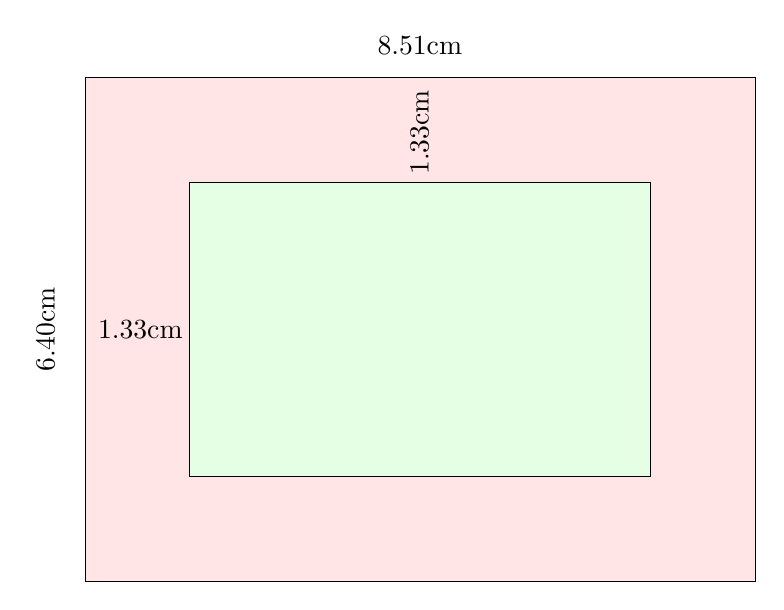
\begin{tikzpicture}
    \filldraw[draw=black, fill=red!10!white] (0cm,0cm) rectangle (8.51cm,6.4cm);
    \filldraw[draw=black, fill=green!10!white] (1.33cm,1.33cm) rectangle 
    (7.18cm,5.06cm);
    \node at (4.25cm, 6.8cm) {8.51cm};
    \node[rotate=90] at (-0.5cm, 3.2cm) {6.40cm};
    \node[rotate=90] at (4.25cm, 5.7cm) {1.33cm};
    \node at (0.7cm, 3.2cm) {1.33cm};
  \end{tikzpicture}
  \label{fig.Schema_Tapis}
  \captionof{figure}{Zones du tapis roulant}
\end{minipage}

\vspace{2cm}
\begin{minipage}[c]{\textwidth}
  \centering
  \begin{tikzpicture}
    \draw (0cm,0cm) rectangle (8.6cm,6.5cm);
  \end{tikzpicture}
  \label{fig.Schema_Tapis}
  \captionof{figure}{Template du tapis}
\end{minipage}